\documentclass[10pt,a4paper,notitlepage]{scrartcl}
\usepackage[utf8]{inputenc}
\usepackage[T1]{fontenc}		% Allow underscore in text
\usepackage[english]{babel}
\usepackage{amsmath}
\usepackage{amsfonts}
\usepackage{amssymb}
\usepackage{graphicx}
\usepackage[obeyspaces]{url}
\usepackage[os=win]{menukeys}
\usepackage{float}
\usepackage[font=small,labelfont=bf]{caption}
\usepackage{listings}
\usepackage{color}
\usepackage{wrapfig}
\renewmenumacro{\menu}[>]{roundedmenus}
\graphicspath{ {figures/} }

\definecolor{codegreen}{rgb}{0,0.6,0}
\definecolor{codegray}{rgb}{0.5,0.5,0.5}
\definecolor{codepurple}{rgb}{0.58,0,0.82}
\definecolor{backcolour}{rgb}{0.95,0.95,0.92}
\definecolor{codeorange}{rgb}{0.95,0.45,0}
\lstdefinestyle{mystyle}{
    % backgroundcolor=\color{backcolour},
    commentstyle=\color{codegreen},
    keywordstyle=\color{magenta},
    numberstyle=\tiny\color{codegray},
    stringstyle=\color{codeorange},
    % basicstyle=\footnotesize,
    basicstyle=\ttfamily\small,
    breakatwhitespace=false,
    breaklines=true,
    captionpos=b,
    keepspaces=true,
    % numbers=left,
    % numbersep=5pt,
    showspaces=false,
    showstringspaces=false,
    showtabs=false,
    tabsize=2
}
\lstset{style=mystyle,language=Python}

\newcommand{\scriptpath}{\path{~/sluss/anhe} }
\newcommand{\pythonversion}{2.7.6 }

\author{André Hedlund}
\title{User Guide}
\subtitle{\texttt{copygroups.py} -- v1.0}
\date{\today}


\begin{document}
\maketitle

\section{Introduction} % (fold)
\label{sec:introduction}
\texttt{copygroups.py} provides four functions that can be executed in the Salomé python console. The purpose of the functions is to achieve a more effective workflow with NX as CAD software and Salomé and Code Aster as CAE software. The main idea is to define groups in NX, and when the \texttt{STEP} file is imported to Salomé the groups are automatically created in Salomé. This workflow makes design-analysis iterations more effective since the user can make changes to the model in NX and these changes are easily imported to Salomé without having to manually recreate groups and mesh definitions.
% section introduction (end)

\section{Installation \& Prerequisites}
The latest version is found in \scriptpath. There are two ways to install the script. Note that a welcome message should be displayed in the Python console after both of these processes. Execute \texttt{help(cg)} in the console to see if the installation process succeeded. Note that the script is written in Python \pythonversion and requires at least Salomé version 7.2 (all testing has been done with version 7.4).

\textbf{Important!} Always load the script \textit{after} the \texttt{STEP} file has been loaded \underline{or} start a new session with \keys{\ctrl+N} and \textit{then} load the script.

\subsection*{Alternative 1} % (fold)
\label{sub:alternative_1}
\begin{enumerate}
    \item Open Salomé.
    \item Press \keys{\ctrl+T} to import a script and browse to the path where the script
is saved.
\end{enumerate}
This installation process needs to be performed every time Salomé is started.
% subsection alternative_1 (end)

\subsection*{Alternative 2} % (fold)
\label{sub:alternative_2}
\begin{enumerate}
    \item Copy copygroups.py to the Salomé folder for python scripts: \\ \path{cp} \scriptpath\path{/copygroups.py /opt/salomemecca2015_1/V2015_1/modules/KERNEL_V7_5_1/lib/python2.7/site-packages/salome}
    \item Open Salomé and start a new Geometry session.
    \item In the Python console type \texttt{from copygroups import *}.
\end{enumerate}
With this installation process the script is automatically executed when Salomé is started, but step 3 needs to be performed every time Salomé is restarted.
% subsection alternative_2 (end)

\section{Usage} % (fold)
\label{sec:usage}
\subsection*{Basics} % (fold)
\label{sub:basics}
Four functions are provided by the script:
\begin{itemize}
	\item \texttt{CreateGroups} (\texttt{cg})
	\item \texttt{PartitionShapes} (\texttt{ps})
	\item \texttt{CreateMesh} (\texttt{cm})
	\item \texttt{CreateSubMesh} (\texttt{csm})
\end{itemize}
A short description and the available input arguments can be obtained by executing \texttt{help(FunctionName)}. All functions can be executed in the python console by their respective abbreviation.

When the input argument to a function is an object in the Object Browser the object name must be specified as \texttt{['ObjectName1','ObjectName2',...]} in the argument list. A convenient alternative is to leave the argument list empty and select the respective objects in the Object Browser instead.

To enable the script to function as intended the groups that are created in NX need to follow a naming convention. Suppose we have two objects that are in contact and that they are exposed to some load condition. The naming convention is as follows:
\begin{itemize}
	\item The objects are given a name with exactly two capital characters, eg. \texttt{AA} and \texttt{BB}.
	\item The contact surface is named by the objects that are in contact separated by an underscore, eg. \texttt{AA\_BB}. If several contact surfaces exist they are given a number suffix, eg. \texttt{AA\_BB1}, \texttt{AA\_BB2}, etc.
	\item A load case (or something else) that is related to a specific object is given the object's name as a prefix, eg. \texttt{AALOAD}.
	\item A group that is intended for local mesh refinements should be given the prefix \texttt{FIN}, eg. \texttt{FINSURFACE}.
\end{itemize}

% subsection basics (end)
\subsection*{\texttt{CreateGroups}} % (fold)
\label{sub:create_groups}
This functions identifies the groups that were defined in NX and creates them in Salomé. The default argument list is given by:
\begin{lstlisting}
	CreateGroups(shape=[], edge=True, vertex=False)
\end{lstlisting}
where \texttt{shape} is the imported \texttt{STEP} file and \texttt{edge}/\texttt{vertex} determine if these respective type of groups should be created (for large models it can be very time consuming to search every vertex of the model, therefore \texttt{vertex} default value is \texttt{False}).
% subsection create_groups (end)

\subsection*{\texttt{PartitionShapes}} % (fold)
\label{sub:partition_shapes}
This function partitions the specified objects and creates a tree structure of the groups that are defined. This tree structure is necessary for the Projection algorithm, which can create a conformal mesh at a contact surface. The default argument list is given by:
\begin{lstlisting}
	PartitionShapes(shapes=[])
\end{lstlisting}
where \texttt{shape} is the objects in the Object Browser that should be partitioned. The resulting tree structure in the Object Browser is shown in Figure~\ref{fig:treestructure}.
\begin{figure}[H]
	\centering
	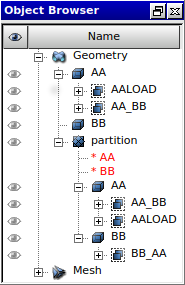
\includegraphics{treestructure}
	\caption{\texttt{PartitionShapes} creates a tree structure of the groups.}
	\label{fig:treestructure}
\end{figure}
% subsection partition_shapes (end)

\subsection*{\texttt{CreateMesh}} % (fold)
\label{sub:create_mesh}
This function creates a hypothesis of the NETGEN meshing algorithm for a specified object in the Object Browser. The hypothesis is created with default values for max and min element size, growth rate, element order, etc. The default argument list is given by:
\begin{lstlisting}
	CreateMesh(shape=[], minSize=10, maxSize=50)
\end{lstlisting}
where \texttt{shape} is the objects in the Object Browser that should be meshed. Note that the mesh is not computed.
% subsection create_mesh (end)

\subsection*{\texttt{CreateSubMesh}} % (fold)
\label{sub:create_sub_mesh}
\begin{wrapfigure}[27]{r}{0.5\textwidth}
	\centering
	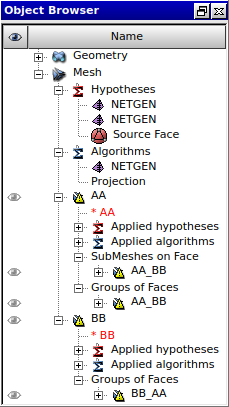
\includegraphics{mesh}
	\caption{\texttt{CreateMesh} and \texttt{CreateSubMesh} creates the necessary mesh algorithms and hypotheses.}
	\label{fig:mesh}
\end{wrapfigure}
This function creates a conformal mesh for contact surfaces as a sub mesh under one of the objects that are in contact. The default argument list is given by:
\begin{lstlisting}
	CreateSubMesh(sourceFace=[])
\end{lstlisting}
where \texttt{sourceFace} is the group in the Object Browser that represent the contact surface (or edge).

As is described in Section~\ref{sub:partition_shapes}, the objects that are in contact need to be partitioned and the groups must be organised in a tree structure. It is therefore necessary to first execute \texttt{PartitionShapes}, then \texttt{CreateMesh} on the objects that are in contact and finally execute \texttt{CreateSubMesh}. This procedure meshes all objects and creates a conformal contact mesh at the contact surface, see Figure~\ref{fig:mesh}.

% subsection create_sub_mesh (end)
\subsection*{Define groups in NX} % (fold)
\label{sub:define_groups_in_nx}
You can create groups of any type in NX (point, edge, face, solid, etc.). Select the appropriate type in the drop-down menu \menu{Selection Filter} and choose the objects you want to include in the group. Set a name for the objects you have selected by right-clicking on one of the selected objects and select properties, \menu{RMB > Properties}, see Figure~\ref{fig:properties}. The name you set is included in the \texttt{STEP} file and is associated with the objects that you selected.

\begin{figure}[H]
	\centering
	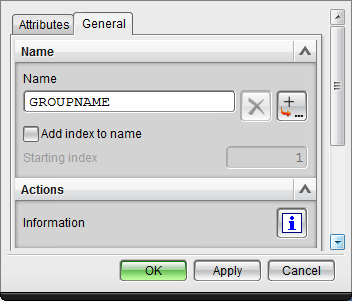
\includegraphics[scale=0.9]{properties}
	\caption{Properties window where the group name is specified.}
	\label{fig:properties}
\end{figure}

Note that an object can not have two names (eg. a face can not be included in a group of faces with name \texttt{GROUPA} and have a separate name \texttt{GROUPB}). For these cases one of the groups have to be created manually in Salomé.
% section usage (end)

\end{document}

